\documentclass[border=10pt]{standalone}
\usepackage{tikz}
\begin{document}
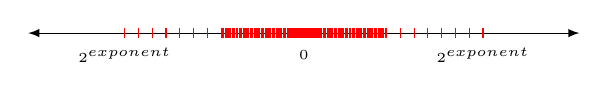
\begin{tikzpicture}[scale=0.35]
  \draw[latex-latex] (-10,0) -- (10,0);
  \foreach \x in {-0.5,-0.48,...,0.5}
    \draw[shift={(\x,0)},color=red] (0pt,5pt) -- (0pt,-5pt);
  \foreach \x in {-3,-2.95,...,3}
    \draw[shift={(\x,0)},color=red] (0pt,5pt) -- (0pt,-5pt);
  \foreach \x in {-6.5,-6.0,...,6.5}
    \draw[shift={(\x,0)},color=red] (0pt,5pt) -- (0pt,-5pt);
  \node[font=\tiny] at (-6.5,-0.8) {$2^{exponent}$};
  \node[font=\tiny] at (0,-0.8) {0};
  \node[font=\tiny] at (6.5,-0.8) {$2^{exponent}$};
\end{tikzpicture}
\end{document}
